\documentclass{article}
\usepackage[utf8]{inputenc}


%%  PACKAGES
%\usepackage{jmbarrett}
\usepackage{amsmath}
\usepackage{amssymb}
\usepackage{amsthm}
\usepackage{enumitem}
\usepackage{hyperref}
\usepackage{parskip}    % remove paragraph indents
\usepackage{stmaryrd}   % for \llbracket and \rrbracket
\usepackage{tikz-cd}
\usepackage{tkz-graph}  % for drawing groupoids
\usepackage[nottoc]{tocbibind}
\usepackage{url}
\usepackage{xcolor}


%%  THEOREMS
\theoremstyle{definition}
\newtheorem{definition}{Definition}[section]
\newtheorem{proposition}[definition]{Proposition}
\newtheorem{remark}[definition]{Remark}


% List stuff
\setlist[itemize,2]{label=$\rhd$}


%%  MACROS

% Type theory
\newcommand{\proves}{\vdash}
\renewcommand{\int}[1]{\mathopen{}\left\llbracket #1
    \right\rrbracket\mathclose{}}       % Interpretation of syntax in model
\newcommand{\emp}{()}%{\mathtt{empty}}          % Empty context
\newcommand{\Bool}{\mathtt{Bool}}
\newcommand{\String}{\mathtt{String}}
\newcommand{\Pii}[2]{\textstyle\prod_{#1} #2}             % Pi type
\newcommand{\lam}[2]{\lambda #1 \mapsto #2}
\newcommand{\Sig}[2]{\textstyle\sum_{#1} #2}              % Sigma type
\newcommand{\refl}{\mathsf{refl}}
\newcommand{\tproj}{\mathsf{pr}}

% Substitutions
\newcommand{\comp}[2]{#2#1}%{#1#2}                     % Composition of substitutions
\newcommand{\substType}[2]{#2#1}%{#1(#2)}              % Substitution on types
\newcommand{\substTerm}[2]{#2#1}%{#1(#2)}              % Substitution on terms
\newcommand{\extsub}[2]{\ang{#1,#2}}

% Categories & functors
\newcommand{\C}{\mathbf{Ctx}}
\newcommand{\Fam}{\mathbf{Fam}}
\newcommand{\Set}{\mathbf{Set}}
\newcommand{\Gpd}{\mathbf{Gpd}}
\newcommand{\Cat}{\mathbf{Cat}}
\newcommand{\Ty}{\mathrm{Ty}}
\newcommand{\Tm}{\mathrm{Tm}}
\newcommand{\op}[1]{{#1}^\mathrm{op}}           % Dual category
\DeclareMathOperator{\Hom}{Hom}

% Groupoids
\newcommand{\G}{\mathcal{G}}
\newcommand{\Hh}{\mathcal{H}}
\DeclareMathOperator{\ob}{ob}
\renewcommand{\hom}[3][]{\mathrm{hom}_{#1}\mathopen{}\left( #2, #3 \right)\mathclose{}}
%{\mathopen{}\left( #2 =_{#1} #3 \right)\mathclose{}}
\newcommand{\inv}[1]{#1^{-1}}
\newcommand{\gfunc}[1]{\overline{#1}}

% Misc math
\newcommand{\N}{\mathbb{N}}		        	    % Natural numbers
\newcommand{\R}{\mathbb{R}}		        	    % Real numbers
\DeclareMathOperator{\id}{id}				    % Identity function
\newcommand{\defeq}{
	\mathrel{\mathrel{\mathop:}\mkern-1.2mu=}}	% := symbol
\newcommand{\tup}[1]{\overline{\smash{#1}\vphantom{a}}}
\newcommand{\ang}[1]{\mathopen{}\left\langle #1 \right\rangle\mathclose{}}
\newcommand{\pair}[2]{(#1,#2)}
\newcommand{\sproj}{\pi}

% Formatting
\newcommand{\n}{%\hspace{-0.2em}
}                % remove space between [[ ]] and ()


\title{Categories with families}
\author{Jordan Mitchell Barrett}
\date{Originally published: {\color{red}\label{todo:date} \today} \\[2mm] This version: \today}

\begin{document}

\maketitle
\tableofcontents


{\color{red}
\section*{To do}

Fill in Appendix \ref{app:gpd}

Interpret path induction in \S\ref{sec:gpd-eq}

Fill in \hyperref[todo:date]{\underline{date}} on title page
}





\section{Introduction}

This report aims to provide a gentle introduction to \textbf{semantics of type theory} and \textbf{categories with families} (CwFs). I've found that existing presentations of this material tend to be terse and mathematically minimal. Of course, this is an efficient way to present that information to experts in the field. However, it assumes context and background which beginners may not have. Here, we aim to bridge that gap.

We will assume the reader has previous exposure to:
\begin{itemize}
    \item Basic type theory, at the level of Chapter 1 of the HoTT book \cite{hottbook}.
    
    \item Category theory, as covered in the first few chapters of your favourite textbook \cite{leinster, maclane}.
\end{itemize}

We'll start by talking about the initial (and possibly canonical) model of type theory, the \textit{syntactic model}, in \S2. This will serve as the primary motivation for the definition of CwFs in \S3. Then, we'll cover two more important models in detail: the \textit{set-theoretical model} in \S4, and Hofmann \& Streicher's \textit{groupoid model} \cite{gpoid} in \S5.

By the end, we hope the reader will be able to make sense of other presentations of CwFs in the literature. Let's dive in!


\section{The syntax of a type theory}
\label{sec:syntax}

A \textit{type theory} is a collection of rules for forming \textit{contexts}, \textit{types}, and \textit{terms}. The exact definition of contexts, types and terms depends on the type theory in question. However, the idea is:
\begin{itemize}
    \item Types are like \textit{sets}, and represent the possible kinds of data we can have. For example, $\N$, $\R$, $\Bool$, $\String$ are types.
    
    \item Terms are like \textit{elements}, and represent individual mathematical objects or pieces of data. Terms are allowed to have variables. For example, $3$, $3 + n$, $n^2 + 4$ are all terms (of type $\N$), while $\pi + e + x$ is a term of type $\R$.
\end{itemize}

Generally, each term $t$ is associated with a unique type $A$, and we write $t : A$ to say $t$ has type $A$. We formalise this idea with the notion of a typing judgment.

\begin{definition}
    A \textit{typing judgment} is a string $t : A$, where $t$ is a term and $A$ is a type.
\end{definition}


\subsection{Contexts}

\begin{definition}
    A \textit{context} $\Gamma$ is a sequence of variables and associated typing judgments, i.e.
    $$\Gamma = \big( x_1 : A_1,\ x_2 : A_2,\ \ldots,\ x_n : A_n \big)$$
\end{definition}

In a context $\Gamma$, the $x_i$ are only allowed to be variables, not arbitrary terms. Furthermore, each type $A_i$ is allowed to \textit{depend} on the previous variables $x_i$, so we might write $\Gamma$ more accurately as
\begin{align*}
    \Gamma = \big(\
    x_1 &: A_1,\\
    x_2 &: A_2(x_1),\\
    x_3 &: A_3(x_1,x_2),\\
    &\mathrel{\vdots}\\
    x_n &: A_n(x_1,\ldots,x_{n-1})\ \big)
\end{align*}

We also have a notion of a typing judgment $t : A$ being \textit{valid} in a context $\Gamma$, which we write $\Gamma \proves t : A$. The exact definition of validity is prescribed by the type theory in question, but the idea is that $\Gamma$ gives us enough information to conclude that $t$ has type $A$.

\begin{remark}
    Not every list of typing judgments is a well-formed context---the rules of the type theory tell us which lists are. Generally, the empty context $\emp$ is well-formed, and given a context $\Gamma$, we can instantiate a new variable $x$ and extend it to $( \Gamma,\, x : A )$, where $A$ is a \textit{valid type}\footnote{We will discuss what this means in \S\ref{sec:types-terms}.} in context $\Gamma$.
\end{remark}


\subsection{Substitutions}

Now, we have a notion of substitution, which takes us from one context to another.

% Try to avoid the notation \sigma : \Gamma \to \Delta, as this looks like a typing judgment

\begin{definition}
    Given two contexts
    \begin{align*}
    \Gamma = \big(\ x_1 &: A_1,                             &\Delta = \big(\ y_1 &: B_1,\\
                    x_2 &: A_2(x_1),                        &                y_2 &: B_2(y_1),\\
                    x_3 &: A_3(x_1,x_2),                    &                y_3 &: B_3(y_1,y_2),\\
                    &\mathrel{\vdots}                       &                &\mathrel{\vdots}\\
                    x_n &: A_n(x_1,\ldots,x_{n-1})\ \big)   &                y_m &: B_m(y_1,\ldots,y_{m-1})\ \big)
    \end{align*}
    a \textit{substitution} $\sigma$ from $\Gamma$ to $\Delta$ is a sequence of terms $(s_1, \ldots, s_m)$ such that $$\Gamma \proves s_i : B_i(s_1,\ldots,s_{i-1})$$ for each $i \leq m$.
    
    % \begin{minipage}{0.48\linewidth}
    % \begin{align*}
    % \Gamma = \big(\
    %     x_1 &: A_1,\\
    %     x_2 &: A_2(x_1),\\
    %     x_3 &: A_3(x_1,x_2),\\
    %     &\mathrel{\vdots}\\
    %     x_n &: A_n(x_1,\ldots,x_{n-1})\ \big)
    % \end{align*}
    % \end{minipage}
    % \begin{minipage}{0.48\linewidth}
    % \begin{align*}
    % \Delta = \big(\
    %     y_1 &: B_1,\\
    %     y_2 &: B_2(y_1),\\
    %     y_3 &: B_3(y_1,y_2),\\
    %     &\mathrel{\vdots}\\
    %     y_m &: B_m(y_1,\ldots,y_{m-1})\ \big)
    % \end{align*}
    % \end{minipage}
\end{definition}

Essentially, we are substituting each $y_i$ for $s_i$, hence the name. The intention is that each $s_i$ is a term constructed from variables $x_i$ in $\Gamma$. Here are some simple observations about substitutions:
\begin{itemize}
    \item We can compose substitutions: if $\sigma = (s_i)$ is a substitution from $\Gamma$ to $\Delta$, and $\tau = (t_j)$ is a substitution from $\Delta$ to $\Theta = (z_j : C_j)_{j \leq k}$, then there is a composite substitution $\comp{\sigma}{\tau}$ from $\Gamma$ to $\Theta$, defined by $$\comp{\sigma}{\tau} = \big( t_j[y_i \defeq s_i] \big)$$
    i.e.\ every occurrence of $y_i$ in $t_j$ is substituted by $s_i$.
    
    \item For every context $\Gamma$, there is a trivial substitution from $\Gamma$ to $\Gamma$, defined $\id_\Gamma = (x_1,\ldots,x_n)$. Furthermore, $\id_\Gamma$ is a two-sided identity for composition.
    
    \item It is laborious (though routine) to prove that composition is associative.
\end{itemize}

The astute reader will have noticed from the above observations that we have just formed a \textit{category} $\C$, with contexts as objects and substitutions as morphisms. This category is known as the \textit{category of contexts} or \textit{syntactic category} of the type theory.
 
A final observation to make is that for every context $\Gamma$, there is a unique substitution from $\Gamma$ to the empty context $\emp$, consisting of an empty list of terms. In categorical terms, $\emp$ is a \textit{terminal object} in our category.

% dont mention Product of contexts = concatenation, since this doesn't coincide with products in the categories we give in a model


\subsection{Types and terms}
\label{sec:types-terms}

For every context $\Gamma$, we have a collection $\Ty(\Gamma)$ of \textit{valid types in $\Gamma$}. The notations ``$\Gamma \proves A$'', ``$\Gamma \proves A\ \mathsf{type}$'', or ``$A \in \Ty(\Gamma)$'' may be used to express that $A$ is a valid type in the context $\Gamma$. As usual, the type theory prescribes rules to determine which types are valid in a given context, but the idea is that $A$ can be formed from the types already in $\Gamma$.

Each type $A \in \Ty(\Gamma)$ also has an associated set of \textit{terms} $$\Tm(\Gamma,A) \defeq \{ t \text{ term} \mid \Gamma \proves t : A \}$$

A substitution $\sigma = (s_i)$ from $\Gamma = (x_h : A_h)$ to $\Delta = (y_i : B_i)$ induces a function from $\Ty(\Delta)$ to $\Ty(\Gamma)$, as follows. Given a valid type $A \in \Ty(\Delta)$, replace every occurrence of $y_i$ in $A$ with $s_i$ to get $\substType{\sigma}{A}$. Furthermore, $\sigma$ induces a function from $A$ to $\substType{\sigma}{A}$ in exactly the same way.

\begin{remark}\label{rmk:term-func}
    Some observations:
    
    \begin{itemize}
        \item If $\sigma = \id$, then the function on types (or terms) induced by $\sigma$ is simply the identity function.
        
        \item The function on types (or terms) induced by $\comp{\sigma}{\delta}$ is the composition\footnote{Here, we mean regular function composition in $\Set$.} of that induced by $\sigma$ and that induced by $\delta$.
    \end{itemize}
\end{remark}

You might already notice that this has the structure of a functor. Indeed, we can package it all up nicely in the following way:

\begin{definition}
    $\Fam$ is ``the category of families of sets'', where:
    \begin{itemize}
        \item The objects are families of sets $(A_i)_{i \in I}$ indexed by a set $I$.
        
        \item The morphisms from $(A_i)_{i \in I}$ to $(B_j)_{j \in J}$ consist of a function $f\colon I \to J$, and for each $i$, a function $g_i\colon A_i \to B_{f(i)}$.
    \end{itemize}
\end{definition}

%We understand the index set $I$ to be $\Ty(\Gamma)$ for some context $\Gamma$, and

\begin{definition}
    Define a map $F\colon \op{\C} \to \Fam$ as follows:
    \begin{itemize}
        \item For a context $\Gamma$, $F(\Gamma)$ consists of the sets $\Tm(\Gamma,A)$ indexed by each $A \in \Ty(\Gamma)$.
        
        \item For a substitution $\sigma$ from $\Gamma$ to $\Delta$, $F(\sigma)$ is the map outlined in Remark \ref{rmk:term-func}.
    \end{itemize}
\end{definition}

\begin{proposition}
    $F$ is a functor $\op{\C} \to \Fam$, called the \textit{term functor} $\Tm\colon \op{\C} \to \Fam$.
\end{proposition}


\subsection{Context extension and projection}

Given any context $\Gamma$ and valid type $A$ in $\Gamma$, we can define an \textit{extended context} $(\Gamma,\, x : A)$. This is also sometimes denoted as $\Gamma.A$.

\begin{itemize}
    \item Then, we have a substitution $\pi$ from $(\Gamma,\, x : A)$ to $\Gamma$, defined by substituting each $x_i$ with $x_i$ (and ignoring $x$). We call $\pi$ the \textit{(first) projection}.

    \item Furthermore, we get a term $q \in \Tm \big( (\Gamma,\, x : A), \substType{\pi}{A} \big)$ by $q \defeq x$. We sometimes call $q$ the \textit{second projection}.

    \item Now, given a substitution $\sigma$ from $\Delta$ to $\Gamma$, and a term $t \in \Tm(\Delta, \substType{\sigma}{A})$, we can extend $\sigma$ to a substitution $\extsub{\sigma}{t}$ from $\Delta$ to $(\Gamma,\, x : A)$, where $x$ is substituted by $t$.

    \item What happens if we compose $\extsub{\sigma}{t}$ and $\pi$? Every $x_i$ is replaced by the $i$th term of $\extsub{\sigma}{t}$, which is just the $i$th term of $\sigma$. Hence,
    \begin{equation}\label{eq:proj1}
        \comp{\extsub{\sigma}{t}}{\pi} = \sigma
    \end{equation}

    \item What about if we apply $\extsub{\sigma}{t}$ to $q$? Remember, $q = x$, and the sole occurrence of $x$ is replaced with $t$, so
    \begin{equation}\label{eq:proj2}
        \substTerm{\extsub{\sigma}{t}}{q} = t
    \end{equation}
\end{itemize}
    
\noindent Try to convince yourself that:
\begin{itemize}
    \item $\extsub{\sigma}{t}$ is the unique substitution satisfying equations \eqref{eq:proj1} and \eqref{eq:proj2}.
    
    \item $\extsub{\pi}{q} = \id_{(\Gamma,\, x : A)}$.
    
    \item $\comp{\tau}{\extsub{\sigma}{ t}} = \extsub{ \comp{\tau}{\sigma}}{\big. \substTerm{\tau}{t}}$.
\end{itemize}

We can express all this in a more categorical way. We've essentially defined an isomorphism between the sets
\begin{align*}
    M(\Delta,\Gamma,A)\ &\defeq\ \big\{ \pair{\sigma}{t} \mathrel{\big|} \sigma \text{ subst.}\ \Delta \to \Gamma,\ t \in \Tm(\Delta, \substType{\sigma}{A}) \big\} \\
    \Hom \big( \Delta, (\Gamma,\, x : A) \big)\ &\defeq\ \{ \text{substitutions from } \Delta \text{ to } (\Gamma,\, x : A) \}
\end{align*}
To go from $M(\Delta,\Gamma,A)$ to $\Hom \big( \Delta, (\Gamma,\, x : A) \big)$, we use the extended substitution as defined above, while in the other direction, we compose with $\pi$ and $q$.

Both of these can be considered as functors $\op{\C} \to \Set$
\begin{align*}
    M(-,\Gamma,A)&\colon\ \Delta\ \mapsto\ M(\Delta,\Gamma,A) \\
    \Hom \big( -, (\Gamma,\, x : A) \big)&\colon\ \Delta\ \mapsto\ \Hom \big( \Delta, (\Gamma,\, x : A) \big)
\end{align*}
with substitutions acting by composition. Now, the isomorphism is a \textit{natural isomorphism} between $M(-,\Gamma,A)$ and $\Hom \big( -, (\Gamma,\, x : A) \big)$ \cite{gpoid}, i.e.\ for every substitution $\tau$ from $\Delta$ to $\Delta'$, the following diagram commutes:
\begin{center}
\begin{tikzcd}[sep=huge]
    \Delta \arrow{d}{\tau} & M(\Delta,\Gamma,A) \arrow{r}{\extsub{\cdot}{\cdot}} & \Hom \big( \Delta, (\Gamma,\, x : A) \big) \\
    \Delta' & M(\Delta',\Gamma,A) \arrow{r}{\extsub{\cdot}{\cdot}} \arrow{u}{\comp{\tau}{(\cdot)}} & \Hom \big( \Delta', (\Gamma,\, x : A) \big) \arrow{u}{\comp{\tau}{(\cdot)}}
\end{tikzcd}
\end{center}

Another nice categorical way to package this up is as follows. Recall that for $\Gamma \in \C$, the \textit{slice category} $\C/\Gamma$ is the category whose:
\begin{itemize}
    \item Objects are substitutions $\sigma\colon \Delta \to \Gamma$, for some $\Delta \in \C$;
    
    \item Morphisms from $\sigma\colon \Delta \to \Gamma$ to $\sigma'\colon \Delta' \to \Gamma$ are substitutions $\tau\colon \Delta \to \Delta'$ such that $\comp{\tau}{\sigma'} = \sigma$.
\end{itemize}

Now, for every $A \in \Ty(\Gamma)$, we can see $M(-,\Gamma,A)$ as a functor $\op{(\C/\Gamma)} \to \Set$, which sends $\sigma\colon \Delta \to \Gamma$ to $\Tm(\Delta,A\sigma)$, and sends morphisms $\tau\colon \Delta \to \Delta'$ to the map they induce on terms (\S\ref{sec:types-terms}). Above, we saw this functor $M$ was naturally isomorphic to the \textit{hom-set functor} $\Hom(-,\pi)\colon \op{(\C/\Gamma)} \to \Set$. This is to say that the projection $\pi$ is a \textit{representing object} for the functor $M$ \cite{nlab-cwfs}.


\section{Categories with families}

Now, we turn to the general idea of a model of type theory. There are many frameworks for defining such models, but we will opt for Dybjer's \textit{categories with families} \cite{peter}.

In fact, we've already seen our first example of a category with families---this was the content of \S\ref{sec:syntax}. This model is known as the \textit{syntactic model} or \textit{term model}. Keeping the syntactic model in mind, hopefully the following definition makes sense.

% The structure should be fully outlined in the previous section before this definition
\begin{definition}\label{defn:cwf}
    A \textit{category with families} (CwF) consists of the following data:
    \begin{itemize}
        \item A \textit{category of contexts} $\C$ with a terminal object $\emp$. % products not required
        
        \item A \textit{term functor} $\Tm\colon \op{\C} \to \Fam$. We will use $\Ty(\Gamma)$ to refer to the index set of $\Tm(\Gamma)$. For a substitution $\sigma$, we write $\substType{\sigma}{A}$ instead of $\Tm(\sigma)(A)$, and $\substType{\sigma}{t}$ instead of $\Tm(\sigma)(t)$.
        
        \item For each context $\Gamma \in \C$ and type $A \in \Ty(\Gamma)$:
        \begin{itemize}
            \item An \textit{extended context} $(\Gamma,\, x : A)$;
            
            \item A substitution $\pi$ from $(\Gamma,\, x : A)$ to $\Gamma$, called the \textit{projection};
            
            \item A term $q \in \Tm \big( (\Gamma,\, x : A), \substType{\pi}{A} \big)$;
        \end{itemize}
        such that for any context $\Delta$, substitution $\sigma$ from $\Delta$ to $\Gamma$, and term $t \in \Tm \big( \Delta, \substType{\sigma}{A} \big)$, there is a unique \textit{extended substitution} $\extsub{\sigma}{t}$ from $\Delta$ to $(\Gamma,\, x : A)$ satisfying
        \begin{align*}
            \comp{\extsub{\sigma}{t}}{\pi} = \sigma & & \substTerm{\extsub{\sigma}{t}}{q} = t
        \end{align*}
    \end{itemize}
\end{definition}

To actually turn a CwF into a fully fledged model of a given type theory, we have to explain how to interpret all of the theory's type- and term-formers (e.g.\ $\to$, $\Pi$, $\Sigma$, $=$, $\lambda$, inductive types, etc). We will do this in more detail for our next example.


\section{Set model}
\label{sec:set}

Let's see our second example of a category with families---the \textit{set-theoretic model} or \textit{set model} \cite{coquand}. This could be considered the ``classical'' model of type theory. The definition of the set model will be informal, and we'll leave it to the reader to formalise it in the style of Definition \ref{defn:cwf}.

For every piece of syntax $S$, we give it an interpretation $\int{S}$ as follows. Given a context\vspace{-3mm}
\begin{align*}
    \Gamma = \big(\
    x_1 &: A_1,\\
    x_2 &: A_2(x_1),\\
    x_3 &: A_3(x_1,x_2),\\
    &\mathrel{\vdots}\\
    x_n &: A_n(x_1,\ldots,x_{n-1})\ \big)
\end{align*}
the type $A_i(x_1,\ldots,x_{i-1})$ is interpreted as a family of sets \textit{indexed by the previous types.} You could also think of this as a \textit{dependent function} of the previous types. So, we have:
\begin{itemize}
    \item A set $\int{A_1}$;
    
    \item For each $a_1 \in \int{A_1}$, a set $\int{A_2}\n(a_1)$;
    
    \item For each $a_1 \in \int{A_1}$ and $a_2 \in \int{A_2}\n(a_1)$, a set $\int{A_3}\n(a_1,a_2)$;
\end{itemize}
and so on.

Then, $\Gamma$ is interpreted as the set $\int{\Gamma}$ of \textit{possible values} for its variables, i.e. $$\int{\Gamma} \defeq \Big\{ (a_1,\ldots,a_n) \mathrel{\Big|} a_i \in \int{A_i}\n(a_1,\ldots,a_{i-1}) \Big\}$$

The empty context is interpreted by a singleton set $\int{\emp} \defeq \{ * \}$.

A substitution $\sigma$ from $\Delta$ to $\Gamma$ is interpreted as a set-theoretic function $\int{\sigma}\colon \int{\Delta} \to \int{\Gamma}$, and composition is the usual function composition.

For every context $\Gamma$, a \textit{type $A$ over $\Gamma$} is a \textit{family of sets} $\int{A}$ indexed by $\int{\Gamma}$. That is, for every possible assignment of variables $(a_1,\ldots,a_n) \in \int{\Gamma}$, we have a set $\int{A}\n(a_1,\ldots,a_n)$. So the collection of types $\Ty(\Gamma)$ over $\Gamma$ is interpreted as $$\int{\big.\Ty(\Gamma)} \defeq \Big\{ \int{A}\colon \int{\Gamma} \to \Set \Big\}$$

Given a type $A \in \Ty(\Gamma)$, a term $t : A$ is interpreted as a \textit{dependent function} $\int{t}$ sending each $(a_1,\ldots,a_n) \in \int{\Gamma}$ to an element $\int{t}\n(a_1,\ldots,a_n) \in \int{A}\n(a_1,\ldots,a_n)$. The collection of terms $\Tm(\Gamma,A)$ is interpreted as the set $\int{\big.\Tm(\Gamma,A)}$ of all such dependent functions.

Now, given a substitution $\sigma\colon \Gamma \to \Delta$, the induced action on types $B \in \Ty(\Delta)$ is $$\int{\big.\substType{\sigma}{B}}\colon\, (a_1,\ldots,a_n)\ \mapsto\ \int{B}\n\big( \sigma(a_1,\ldots,a_n) \big)$$
and on terms $t \in \Tm(\Delta,B)$:
$$\int{\big.\substTerm{\sigma}{t}} :\, (a_1,\ldots,a_n)\ \mapsto\ \int{t}\n\big( \sigma(a_1,\ldots,a_n) \big)$$

Given a context $\Gamma$ and a type $A \in \Ty(\Gamma)$, the extended context $(\Gamma,\, x : A)$ is interpreted as the set
$$\int{\big.(\Gamma,\, x : A)} \defeq \Big\{ (a_1,\ldots,a_n,a) \mathrel{\Big|} (a_1,\ldots,a_n) \in \int{\Gamma},\ a \in \int{A}\n(a_1,\ldots,a_n) \Big\}$$

The projection $\pi$ from $(\Gamma,\, x : A)$ to $\Gamma$ is interpreted simply as the set-theoretic projection
$$\arraycolsep=1.5mm
\begin{array}{rrcl}
    \int{\pi}\colon& \int{\big.(\Gamma,\, x : A)} &\to& \int{\Gamma}\\[1mm]
    \int{\pi}\colon& (a_1,\ldots,a_n,a) &\mapsto& (a_1,\ldots,a_n)
\end{array}$$
while the second projection $q$ is interpreted as the term $\int{q} \in \int{\Tm \big( (\Gamma,\, x : A), \substType{\pi}{A} \big)}$ sending $(a_1,\ldots,a_n,a)$ to $a$.

Given a substitution $\sigma\colon \Delta \to \Gamma$ and term $t \in \Tm \big( \Delta, \substType{\sigma}{A} \big)$, we interpret the extended substitution $\extsub{\sigma}{t}$ as
$$\arraycolsep=1.5mm
\begin{array}{rrcl}
    \int{\big.\extsub{\sigma}{t}}\colon& \int{\Delta} &\to& \int{\big.(\Gamma,\, x : A)} \\[1mm]
    \int{\big.\extsub{\sigma}{t}}\colon& (b_1,\ldots,b_m) &\mapsto& \Big( \int{\sigma}\n(b_1,\ldots,b_m),\, \int{t}\n(b_1,\ldots,b_m) \Big)
\end{array}$$
We leave it to the reader to verify the universal property of $\int{\big.\extsub{\sigma}{t}}$.

At this point, we have fully defined a category with families. For the interested reader, we show in Appendix \ref{app:set} how to interpret $\Pi$-types, $\Sigma$-types and equality in the set model.


\section{Groupoid model}
\label{sec:gpd}

With the set model under our belt, let's move on to another important model---the \textit{groupoid model}. Historically, this model is important because it was the first model of Martin-L\"of type theory in which \textit{uniqueness of identity proofs} (UIP) failed---that is, we can find a type $A$ and elements $a, b : A$ such that $(a = b)$ contains more than one distinct element.

The idea is fairly simple, actually. It has long been observed that the equalities on a type $A$ form a \textit{groupoid} structure on $A$. Hofmann and Streicher's idea was to \textit{interpret} types as groupoids. Then, we can show UIP fails by exhibiting a groupoid with two distinct parallel paths (of which there are many). It is a bit more complex to turn this idea into a full model of MLTT, but we will show how in this section.

The groupoid model is essentially built by ``adding extra structure'' to the set model, so we recommend fully understanding \S\ref{sec:set} before reading this one. For completeness, we'll start by defining groupoids.

\begin{definition}
    A groupoid is a category where every morphism has an inverse. More concretely, a groupoid $\G$ consists of:
    \begin{itemize}
        \item A set $\ob\G$ of \textit{objects of $\G$};
        
        \item For every $a, b \in \ob\G$, a set $\hom{a}{b}$ of \textit{morphisms from $a$ to $b$};
        
        \item For every $a \in \ob\G$, an \textit{identity morphism} $\id_a \in \hom{a}{a}$;
        
        \item For every $a, b \in \ob\G$, an \textit{inverse function} $\inv{(\cdot)}\colon \hom{a}{b} \to \hom{b}{a}$;
        
        \item For every $a, b, c \in \ob\G$, a \textit{composition operation} $\circ\colon \hom{b}{c} \times \hom{a}{b} \to \hom{a}{c}$;
    \end{itemize}
    such that:
    \begin{itemize}
        \item For every $f \in \hom{a}{b}$, $f \circ \id_a = f$ and $\id_b \circ f = f$;
        
        \item For every $f \in \hom{a}{b}$, $\inv{f} \circ f = \id_a$ and $f \circ \inv{f} = \id_b$;
        
        \item For every $f \in \hom{a}{b}$, $g \in \hom{b}{c}$ and $c \in \hom{c}{d}$, $h \circ (g \circ f) = (h \circ g) \circ f$.
    \end{itemize}
\end{definition}

In the context of the groupoid model, a groupoid $\G$ is best understood as a set ($\ob \G$) with extra ``equalities'' (morphisms) imposed on top, where two objects $a$, $b$ are ``equal'' if there is a morphism in $\hom{a}{b}$.

A \textit{groupoid homomorphism} from $\G$ to $\Hh$ is just a functor from $\G$ to $\Hh$, when viewed as categories. Groupoids and groupoid homomorphisms therefore form a full subcategory $\Gpd$ of $\Cat$.

To model \textit{dependent} types using groupoids, we need a notion of a family of groupoids dependent on/indexed by another groupoid. Henceforth, we will abuse notation slightly, and identify a groupoid with its underlying set of objects. Thus, we will use $a \in \G$ to mean $a \in \ob\G$.

\begin{definition}
    Given a groupoid $\G$, a \textit{family of groupoids indexed over $\G$} is a functor $\G \to \Gpd$. More concretely, it consists of:
    \begin{itemize}
        \item For every $a \in G$, a groupoid $\Hh_a$;
        
        \item For every morphism $p \in \hom{a}{b}$, a groupoid homomorphism $F_p\colon \Hh_a \to \Hh_b$;
    \end{itemize}
    so that $F_{\id}$ is the identity homomorphism, and $F_p \circ F_q = F_{(p \circ q)}$.
\end{definition}

The groupoid axioms ensure that each $F_p$ is an isomorphism of groupoids. The intended meaning is that if $a=b$ in $\G$, then the groupoids $\Hh_a$ and $\Hh_b$ are isomorphic.

Now, we're ready to define the groupoid model. For every piece of syntax $S$, we give it an interpretation $\int{S}$ as follows. Given a context%\vspace{-6mm}
\begin{align*}
    \Gamma = \big(\
    x_1 &: A_1,\\
    x_2 &: A_2(x_1),\\
    x_3 &: A_3(x_1,x_2),\\
    &\mathrel{\vdots}\\
    x_n &: A_n(x_1,\ldots,x_{n-1})\ \big)
\end{align*}
the type $A_i(x_1,\ldots,x_{i-1})$ is interpreted as a family of \textit{groupoids} indexed by the previous types. As in the set model, we have:
\begin{itemize}
    \item A groupoid $\int{A_1}$;
    
    \item For each $a_1 \in \int{A_1}$, a groupoid $\int{A_2}\n(a_1)$;
    
    \item For each $a_1 \in \int{A_1}$ and $a_2 \in \int{A_2}\n(a_1)$, a groupoid $\int{A_3}\n(a_1,a_2)$;
\end{itemize}
and so on. But, additionally, the equalities in earlier types induce \textit{coherences} in the later types:

\begin{itemize}
    \item For each $\int{A_1}$-morphism $p_1 \in \hom{a_1}{b_1}$,\\ we get a groupoid isomorphism $\gfunc{p_1}\colon \int{A_2}\n(a_1) \to \int{A_2}\n(b_1)$;
    
    \item For each $\int{A_1}$-morphism $p_1 \in \hom{a_1}{b_1}$\\ and $\int{A_2}\n(b_1)$-morphism $p_2 \in \hom{\gfunc{p_1} a_2}{b_2}$,\\ we get a groupoid isomorphism $\gfunc{p_1p_2}\colon \int{A_3}\n(a_1,a_2) \to \int{A_3}\n(b_1,b_2)$;
\end{itemize}
and so on.

As in the set model, $\Gamma$ is interpreted as the set $\int{\Gamma}$ of \textit{possible values} for its variables: $$\int{\Gamma} \defeq \Big\{ (a_1,\ldots,a_n) \mathrel{\Big|} a_i \in \int{A_i}\n(a_1,\ldots,a_{i-1}) \Big\}$$

The morphisms of $\int{\Gamma}$ are those induced by the groupoid structure on each of the $\int{A_i}$:
\begin{align*}
    \hom[\int{\Gamma}]{\big.(a_1,\ldots,a_n)}{(b_1,\ldots,b_n)}\\ \defeq\ \big\{ (p_1, \ldots, p_n)& \mathrel{\big|} p_i \in \hom{\gfunc{p_1 \cdots p_{i-1}} a_i}{b_i} \big\}
\end{align*}

\vspace{-2mm}
\begin{minipage}[b]{0.83\linewidth}
The empty context is interpreted by the trivial groupoid with one object and one identity morphism, as shown on the right.
\end{minipage}
\hfill
\begin{minipage}[b]{0.12\linewidth}
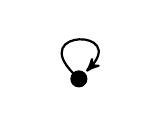
\begin{tikzpicture}[scale=1]
    \GraphInit[vstyle=Classic]
    \SetVertexSimple[MinSize=1mm]
    \Vertex[NoLabel]{A}
    \Loop[dist=8mm,dir=NO%label=$\id$,labelstyle={above}
    ](A)
\end{tikzpicture}
\end{minipage}


A substitution $\sigma$ from $\Delta$ to $\Gamma$ is interpreted as a groupoid homomorphism $\int{\sigma}\colon \int{\Delta} \to \int{\Gamma}$.

Henceforth, we will abbreviate $(a_1,\ldots,a_n) \in \int{\Gamma}$ as $\tup{a}$. For a context $\Gamma$, a \textit{type $A$ over $\Gamma$} is a family of \textit{groupoids} $\int{A}$ indexed by $\int{\Gamma}$. That is:
\begin{itemize}
    \item For every $\tup{a} \in \int{\Gamma}$, we have a groupoid $\int{A}(\tup{a})$;
    
    \item For every $\int{\Gamma}$-morphism $p \in \hom{\tup{a}}{\tup{b}}$, a groupoid isomorphism $\int{A}(p)\colon \int{A}(\tup{a}) \to \int{A}(\tup{b})$, such that:
    \begin{itemize}
        \item $\int{A}(\id_{\tup{a}}) = \id_{\int{A}(\tup{a})}$;
        
        \item $\int{A}(p \circ q) = \int{A}(p) \circ \int{A}(q)$.
    \end{itemize}
\end{itemize}

For a type $A$ over $\Gamma$, a term $s \in \Tm(\Gamma,A)$ is interpreted as a ``dependent functor'' $\int{\Gamma} \to \int{A}$:
\begin{itemize}
    \item For each $\tup{a} \in \int{\Gamma}$, we have an object $\int{s}(\tup{a}) \in \int{A}(\tup{a})$;
    
    \item For each $\int{\Gamma}$-morphism $p \in \hom{\tup{a}}{\tup{b}}$, an $\int{A}(\tup{b})$-morphism $$\int{s}(p)\, \in\, \hom{\Big.\int{A}(p) \big( \int{s}(\tup{a}) \big)}{\,\int{s}(\tup{b})}$$
    such that:
    \begin{itemize}
        \item $\int{s}(\id_{\tup{a}}) = \id_{\int{s}(\tup{a})}$;
        
        \item $\int{s}(p \circ q) = \int{s}(p) \circ \int{A}(p) \big( \int{s}(q) \big)$.
    \end{itemize}
\end{itemize}

Given a substitution $\sigma\colon \Gamma \to \Delta$ and a type $B \in \Ty(\Delta)$, we interpret $\substType{\sigma}{B} \in \Ty(\Gamma)$ as follows. $\int{\substType{\sigma}{B}}$ sends:
\begin{itemize}
    \item $\tup{a} \in \int{\Gamma}$ to the groupoid $\int{B}(\sigma(\tup{a}))$;
    
    \item $p \in \hom[\int{\Gamma}]{\tup{a}}{\tup{b}}$ to the homomorphism $\int{B}(\sigma(p))\colon \int{B}(\sigma(\tup{a})) \to \int{B}(\sigma(\tup{b}))$.
\end{itemize}

Similarly, for $t \in \Tm(\Delta,B)$, we interpret $\substTerm{\sigma}{t} \in \Tm(\Gamma,\substType{\sigma}{B})$ as the map $\int{\substTerm{\sigma}{t}}$ sending:
\begin{itemize}
    \item $\tup{a} \in \int{\Gamma}$ to the object $\int{t}(\sigma(\tup{a})) \in \int{B}(\sigma(\tup{a}))$;
    
    \item $p \in \hom[\int{\Gamma}]{\tup{a}}{\tup{b}}$ to the $\int{B}(\sigma(\tup{b}))$-morphism $$\int{t}(\sigma(p))\, \in\, \hom{\Big.\int{B}(\sigma(p)) \big( \int{t}(\sigma(\tup{a})) \big)}{\,\int{t}(\sigma(\tup{b}))}$$
\end{itemize}

Given a context $\Gamma$ and a type $A \in \Ty(\Gamma)$, the extended context $(\Gamma,\, x : A)$ is interpreted as the groupoid with objects
$$\int{\big.\Gamma,\, x : A} \defeq \big\{ (\tup{a},a) \mathrel{\big|} \tup{a} \in \int{\Gamma},\ a \in \int{A}(\tup{a}) \big\}$$
and morphisms
\begin{align*}
    \hom[\int{\Gamma,\, x : A}]{\big.(\tup{a},a)}{(\tup{b},b)}\ \defeq\ \Big\{ (p,p') \mathrel{\Big|}\ &p \in \hom[\int{\Gamma}]{\tup{a}}{\tup{b}},\\[-2mm]
    &p' \in \hom[\int{A}(\tup{b})]{\big.\int{A}(p)(a)}{\,b} \Big\}
\end{align*}

The projection $\pi$ from $(\Gamma,\, x : A)$ to $\Gamma$ is interpreted as the groupoid homomorphism sending $(\tup{a},a)$ to $\tup{a}$, and $(p,p')$ to $p$. Similarly, the second projection $q$ is interpreted as the term $\int{q} \in \int{\Tm \big( (\Gamma,\, x : A), \substType{\pi}{A} \big)}$ sending $(\tup{a},a)$ to $a$, and $(p,p')$ to $p'$.

Finally, given a substitution $\sigma\colon \Delta \to \Gamma$ and term $t \in \Tm \big( \Delta, \substType{\sigma}{A} \big)$, we interpret the extended substitution $\extsub{\sigma}{t}: \Delta \to (\Gamma,\, x : A)$ as follows:
\begin{itemize}
    \item $\int{\extsub{\sigma}{t}}$ maps $\tup{c} \in \int{\Delta}$ to $\big( \int{\sigma}(\tup{c}), \int{t}(\tup{c}) \big) \in \int{\Gamma,\, x : A}$.
    
    \item $\int{\extsub{\sigma}{t}}$ maps $p \in \hom[\int{\Delta}]{\tup{c}}{\tup{d}}$ to $\big( \int{\sigma}(p), \int{t}(p) \big)$.
\end{itemize}


\subsection{Equality}
\label{sec:gpd-eq}

We have now fully defined a category with families. We will leave the interpretation of $\Pi$-types and $\Sigma$-types to Appendix \ref{app:gpd}. However, we will talk here about \textit{equality types}, since they are the original motivation (and arguably, the defining feature) of the groupoid model.

Given a type $A \in \Ty(\Gamma)$ and terms $s, t \in \Tm(\Gamma, A)$, the equality type $(s =_A t) \in \Ty(\Gamma)$ is interpreted as the \textit{hom-set}
$$\int{\big.s =_A t}\n(\tup{a})\, \defeq\, \hom[\int{A}(\tup{a})]{\big.\int{s}(\tup{a})}{\int{t}(\tup{a})}$$
as a \textit{discrete} groupoid (i.e.\ the only morphisms are identities).

Given $s \in \Tm(\Gamma,A)$, we interpret $\refl_s \in \Tm\big(\Gamma, (s =_A s) \big)$ as $$\int{\refl_s}\colon\, \tup{a}\, \mapsto\, \id_{\int{s}(\tup{a})}$$

{\color{red} Check rules}

Importantly, since there are groupoids having distinct parallel morphisms, there are types in this model having distinct equalities between two elements. Therefore, the groupoid model provides a counterexample to UIP.


\section{Conclusion}

We have now seen three models of type theory---the syntactic model (\S\ref{sec:syntax}), the set model (\S\ref{sec:set}), and the groupoid model (\S\ref{sec:gpd}). There are many, many other models of type theory, such as the setoid model \cite{setoid}, the $\omega$-groupoid model \cite{om-gpoid}, presheaf models \cite{huber} and more. We hope that the reader will now be equipped to read and understand the existing presentations of these models in the literature.


\begin{thebibliography}{9}

\bibitem{coquand} Thierry Coquand. \textit{What is a model of type theory?} Notes from the Special Year on Univalent Foundations of Mathematics, Institute for Advanced Study, Princeton, 2012. \url{https://ncatlab.org/ufias2012/files/cwf1.pdf}

\bibitem{peter} Peter Dybjer. \textit{Internal type theory.} pp120--134 in: Stefano Berardi, Mario Coppo (eds.), \textit{Types for Proofs and Programs} (proceedings from TYPES '95, Torino, Italy, June 1995). Lecture Notes in Computer Science \textbf{1158}, Springer, 1996. Available online at \url{https://www.cse.chalmers.se/~peterd/papers/InternalTT.pdf}

\bibitem{setoid} Martin Hofmann. \textit{Extensional concepts in intensional type theory}. PhD thesis, University of Edinburgh, 1995.

\bibitem{gpoid} Martin Hofmann, Thomas Streicher. \textit{The groupoid interpretation of type theory.} pp83--112 in: Giovanni Sambin, Jan M.\ Smith (eds.), \textit{Twenty Five Years of Constructive Type Theory} (conference proceedings from Venice, October 1995). Oxford Logic Guides \textbf{36}, Oxford University Press, 1998.

\bibitem{huber} Simon Huber. \textit{Cubical interpretations of
type theory}. PhD thesis, University of Gothenburg, 2016.

\bibitem{leinster} Tom Leinster. \textit{Basic Category Theory.} Cambridge Studies in Advanced Mathematics \textbf{143}, Cambridge University Press, 2014. \href{https://arxiv.org/abs/1612.09375}{\texttt{arXiv:1612.09375}}

\bibitem{maclane} Saunders Mac Lane. \textit{Categories for the Working Mathematician.} 2nd ed. Graduate Texts in Mathematics \textbf{5}, Springer, 1998.

\bibitem{om-gpoid} Michael A.\ Warren. \textit{The strict $\omega$-groupoid interpretation of type theory}. pp291--340 in: Centre de Recherches Math\'ematiques Proceedings and Lecture Notes \textbf{53}, 2011.

\bibitem{hottbook} \textit{Homotopy Type Theory:
Univalent Foundations of Mathematics} (a.k.a.\ ``the HoTT book''). 2013. Available at \url{https://homotopytypetheory.org/book/}

\bibitem{nlab-cwfs} The nLab. \textit{Categorical model of dependent types $>$ Categories with families.} \url{https://ncatlab.org/nlab/show/categorical+model+of+dependent+types#categories_with_families}

\bibitem{nlab-synt} The nLab. \textit{Syntactic category.} \url{https://ncatlab.org/nlab/show/syntactic+category}
\end{thebibliography}


\appendix

\section{More on the set model}
\label{app:set}

In this section, we show how to interpret some of the common type- and term-formers in the set model defined in \S\ref{sec:set}. Hence, this should be read directly after that section. Henceforth, we will abbreviate $(a_1,\ldots,a_n) \in \int{\Gamma}$ as $\tup{a}$.


\subsection{\texorpdfstring{$\Pi$}{Pi}-types}

Given a context $\Gamma$ and types $A, B \in \Ty(\Gamma)$, the arrow type $(A \to B) \in \Ty(\Gamma)$ is interpreted as the family
%$$\int{\big.A \to B}\n(a_1,\ldots,a_n)\ \defeq\ \big\{ f\colon \int{A}\n(a_1,\ldots,a_n)\, \to\, \int{B}\n(a_1,\ldots,a_n) \big\} $$
$$\int{\big.A \to B}\n(\tup{a})\ \defeq\ \big\{ \text{functions from}\, \int{A}\n(\tup{a}) \text{ to}\, \int{B}\n(\tup{a}) \big\} $$

More generally, if $A \in \Ty(\Gamma)$ and $B \in \Ty \big( (\Gamma,\, x:A) \big)$, then $\Pii{(x:A)}{B(x)}\in \Ty(\Gamma)$ is interpreted as
\begin{align*}
    \int{\Pii{(x:A)}{B(x)}}(\tup{a})\ \defeq\ \Big\{ \text{functions sending each } a \in &\int{A}\n(\tup{a}) \\[-2mm]
    \text{ to an element of } &\int{B}\n(\tup{a},a) \Big\}
\end{align*}

Given a term $t \in \Tm \big( (\Gamma,\, x:A), B \big)$, the lambda abstraction $(\lam{(x:A)}{t}) \in \Tm\big( \Gamma, \Pii{(x:A)}{B(x)} \big)$ is interpreted as
$$\int{\big.\lam{(x:A)}{t}}\n(\tup{a})\ \defeq\ a %\in \int{A}\n(\tup{a})
\mapsto \int{t}\n(\tup{a},a)$$

Now, given a term $s \in \Tm(\Gamma, A)$, we write $B(s) \defeq \substType{(\id,s)}{B} \in \Ty(\Gamma)$, where $\extsub{\id}{s}$ is the extended substitution $\Gamma \to (\Gamma,\, x:A)$. Given another term $f \in \Tm\big( \Gamma, \Pii{(x:A)}{B(x)} \big)$, the application $f(s) \in \Tm\big(\Gamma,B(s) \big)$ is interpreted as
$$\int{\big.f(s)
}\n(\tup{a})\ \defeq\ \int{f}\n(\tup{a}) \big( \int{s}\n(\tup{a}) \big)$$

Letting $t(s) \defeq \substTerm{\extsub{\id}{s}}{t} \in \Ty\big(\Gamma,B(s)\big)$, the computation rule $$(\lam{(x:A)}{t})(s)\ \equiv\ t(s)$$ holds since both sides are interpreted as $\tup{a}\, \mapsto\, \int{t}\n\big(\tup{a}, \int{s}\n(\tup{a}) \big)$.

Given $f \in \Tm\big( \Gamma, \Pii{(x:A)}{B(x)} \big)$, write $f(x) \in \Tm \big( (\Gamma,\, x:A), B \big)$ for the term interpreted $$\int{\big.f(x)}\n(\tup{a},a)\, \defeq\, \int{f}\n(\tup{a})(a)$$
Then $\int{\big.\lam{(x:A)}{f(x)}} = \int{f}$, validating the uniqueness rule $$\big( \lam{(x:A)}{f(x)} \big) \equiv f$$


\subsection{\texorpdfstring{$\Sigma$}{Sigma}-types}

Given a context $\Gamma$ and types $A, B \in \Ty(\Gamma)$, the product type $(A \times B) \in \Ty(\Gamma)$ is interpreted as the family
%$$\int{\big.A \to B}\n(a_1,\ldots,a_n)\ \defeq\ \big\{ f\colon \int{A}\n(a_1,\ldots,a_n)\, \to\, \int{B}\n(a_1,\ldots,a_n) \big\} $$
$$\int{\big.A \times B}\n(\tup{a})\ \defeq\ \int{A}\n(\tup{a}) \times \int{B}\n(\tup{a})$$

More generally, if $A \in \Ty(\Gamma)$ and $B \in \Ty \big( (\Gamma,\, x:A) \big)$, then $\Sig{(x:A)}{B(x)}\in \Ty(\Gamma)$ is interpreted as
\begin{align*}
    \int{\Sig{(x:A)}{B(x)}}(\tup{a})\ \defeq\ \big\{ (a,b) \mathrel{\big|} a \in &\int{A}\n(\tup{a}),\ b \in \int{B}\n(\tup{a},a) \big\}
\end{align*}

Given terms $s \in \Tm(\Gamma, A)$ and $t \in \Tm \big( (\Gamma,\, x:A), B \big)$, the pair $(s,t) \in \Tm\Big( \Gamma, \Sig{(x:A)}{B(x)} \Big)$ is interpreted as
$$\int{\big.(s,t)}\n(\tup{a})\ \defeq\ \Big( \int{s}\n(\tup{a}),\ \int{t}\n\big(\, \tup{a},\,\int{s}\n(\tup{a}) \,\big) \Big)$$

Given a term $u \in \Tm\Big( \Gamma, \Sig{(x:A)}{B(x)} \Big)$, we interpret the first projection $\tproj_1(u) \in \Tm(\Gamma, A)$ as $$\int{\big.\tproj_1(u)}(\tup{a})\, \defeq\, \text{first coordinate of } \int{u}(\tup{a})$$%\sproj_1 \big( \int{u}(\tup{a}) \big)$$
and the second projection $\tproj_2(u) \in \Tm \Big( \Gamma, B \big( \tproj_1(u) \big) \Big)$ as $$\int{\big.\tproj_2(u)}(\tup{a})\, \defeq\, \text{second coordinate of } \int{u}(\tup{a})$$%\sproj_2 \big( \int{u}(\tup{a}) \big)$$
%where $\sproj_1$, $\sproj_2$ are the usual set-theoretic projections.
These interpretations validate the computation rules
\begin{align*}
    \tproj_1 \big( (s,t) \big) \equiv s & & \tproj_2 \big( (s,t) \big) \equiv t & & \big( \tproj_1(u), \tproj_2(u) \big) \equiv u
\end{align*}


\subsection{Equality}

Perhaps the distinguishing feature of the set model is its treatment of equality types. Unlike in other models, equality here behaves exactly like a classical mathematician would expect.

Given a type $A \in \Ty(\Gamma)$ and terms $s, t \in \Tm(\Gamma, A)$, the equality type $(s =_A t) \in \Ty(\Gamma)$ is interpreted as
$$\int{\big.s =_A t}\n(\tup{a}) \defeq \begin{cases}
    \{ * \} & \int{s}(\tup{a}) = \int{t}(\tup{a}) \\
    \varnothing & \text{otherwise}
\end{cases}$$

Given $s \in \Tm(\Gamma,A)$, we interpret $\refl_s \in \Tm\big(\Gamma, (s =_A s) \big)$ as $\int{\refl_s}(\tup{a}) = *$.

Path induction is straightforward to interpret, as the only values of equality in this model are $\refl$.


\section{More on the groupoid model}
\label{app:gpd}

In this section, we show how to interpret $\Pi$-types and $\Sigma$-types in the groupoid model, as defined in \S\ref{sec:gpd}. This section should be read after \S\ref{sec:set}, \S\ref{sec:gpd} and Appendix \ref{app:set}. As in the previous appendix, we will abbreviate $(a_1,\ldots,a_n) \in \int{\Gamma}$ as $\tup{a}$.


\subsection{\texorpdfstring{$\Pi$}{Pi}-types}

{\color{red} finish this}


\subsection{\texorpdfstring{$\Sigma$}{Sigma}-types}

Given a context $\Gamma$ and types $A, B \in \Ty(\Gamma)$, the product type $(A \times B) \in \Ty(\Gamma)$ is interpreted as the family
%$$\int{\big.A \to B}\n(a_1,\ldots,a_n)\ \defeq\ \big\{ f\colon \int{A}\n(a_1,\ldots,a_n)\, \to\, \int{B}\n(a_1,\ldots,a_n) \big\} $$
$$\int{\big.A \times B}\n(\tup{a})\ \defeq\ \int{A}\n(\tup{a}) \times \int{B}\n(\tup{a})$$
with morphisms
\begin{align*}
    \hom[\int{A \times B}(\tup{a})]{\big.(a,b)}{(a',b')}\\ \defeq\ \big\{ (p,q)& \mathrel{\big|} p \in \hom[\int{A}(\tup{a})]{a}{a'},\, q \in \hom[\int{B}(\tup{a})]{b}{b'} \big\}
\end{align*}

%A $\int{\Gamma}$-morphism $r \in \hom%[\int{\Gamma}]
%{\tup{a}}{\tup{b}}$ maps to the groupoid homomorphism
% \begin{align*}
%     \int{\big.A \times B}(r)\colon\ \int{\big.A \times B}(\tup{a})\ &\to\ \int{\big.A \times B}(\tup{b}) \\
%     (a,b)\ &\mapsto\ \Big( \int{A}(r)(a),\, \int{B}(r)(b) \Big)
% \end{align*}

More generally, if $A \in \Ty(\Gamma)$ and $B \in \Ty \big( (\Gamma,\, x:A) \big)$, then $\Sig{(x:A)}{B(x)}\in \Ty(\Gamma)$ is interpreted as
\begin{align*}
    \int{\Sig{(x:A)}{B(x)}}(\tup{a})\ \defeq\ \big\{ (a,b) \mathrel{\big|} a \in &\int{A}\n(\tup{a}),\ b \in \int{B}\n(\tup{a},a) \big\}
\end{align*}
with morphisms
\begin{align*}
    \hom%[\int{\Sig{(x:A)}{B(x)}}(\tup{a})]
    {\big.(a,b)}{(a',b')}\ \defeq\ \big\{ (p,q)& \mathrel{\big|} p \in \hom[\int{A}(\tup{a})]{a}{a'},\, q \in \hom[\int{B}(\tup{a},a')]{\big.\int{B}(\id_{\tup{a}},p)(b)}{b'} \big\}
\end{align*}

A $\int{\Gamma}$-morphism $r \in \hom%[\int{\Gamma}]
{\tup{c}}{\tup{d}}$ maps to the groupoid homomorphism
\begin{align*}
    \int{\Sig{(x:A)}{B(x)}}(r)\colon\ \int{\Sig{(x:A)}{B(x)}}(\tup{c})\ &\to\ \int{\Sig{(x:A)}{B(x)}}(\tup{d}) \\[2mm]
    (a,b)\ &\mapsto\ \Big( \int{A}(r)(a),\, \int{B}(r,\id%_{\int{A}(r)(a)}
    )(b) \Big)
\end{align*}

Given terms $s \in \Tm(\Gamma, A)$ and $t \in \Tm \big( (\Gamma,\, x:A), B \big)$, the pair $(s,t) \in \Tm\Big( \Gamma, \Sig{(x:A)}{B(x)} \Big)$ is interpreted as the map sending
\begin{itemize}
    \item $\tup{a} \in \int{\Gamma}$ to $\Big( \int{s}\n(\tup{a}),\ \int{t}\n\big(\, \tup{a},\,\int{s}\n(\tup{a}) \,\big) \Big)$;
    
    \item $p \in \hom[\int{\Gamma}]{\tup{a}}{\tup{b}}$ to $\Big( \int{s}(p),\, \int{t}(p,\id) \Big)$.
\end{itemize}

Given a term $u \in \Tm\Big( \Gamma, \Sig{(x:A)}{B(x)} \Big)$, we interpret the first projection $\tproj_1(u) \in \Tm(\Gamma, A)$ as the map sending
\begin{itemize}
    \item $\tup{a} \in \int{\Gamma}$ to the first coordinate of $\int{u}(\tup{a})$;
    
    \item $p \in \hom[\int{\Gamma}]{\tup{a}}{\tup{b}}$ to the first coordinate of $\int{u}(p)$.
\end{itemize}

We let $B \big( \tproj_1(u) \big) \in \Ty(\Gamma)$ be the type sending
\begin{itemize}
    \item $\tup{a} \in \int{\Gamma}$ to $\int{B} \big( \tup{a},\, \int{\tproj_1(u)}(\tup{a}) \big)$;
    
    \item $p \in \hom[\int{\Gamma}]{\tup{a}}{\tup{b}}$ to $\int{B} \big( p,\, \int{\tproj_1(u)}(p) \big)$.
\end{itemize}
Then, the second projection $\tproj_2(u) \in \Tm \Big( \Gamma, B \big( \tproj_1(u) \big) \Big)$ is interpreted as the map sending
\begin{itemize}
    \item $\tup{a} \in \int{\Gamma}$ to the second coordinate of $\int{u}(\tup{a})$;
    
    \item $p \in \hom[\int{\Gamma}]{\tup{a}}{\tup{b}}$ to the second coordinate of $\int{u}(p)$.
\end{itemize}

These interpretations validate the computation rules
\begin{align*}
    \tproj_1 \big( (s,t) \big) \equiv s & & \tproj_2 \big( (s,t) \big) \equiv t & & \big( \tproj_1(u), \tproj_2(u) \big) \equiv u
\end{align*}


\end{document}
